\section{连续釜式反应器的定态操作}


\begin{frame}
    \frametitle{连续釜式反应器的定态操作}

    \large 连续釜式反应器内反应物料温度均匀一致，若为定态操作，反应是在等温下进行的。如为非定态操作，仍属变温过程，即反应温度系随时间而变，但不随空间而变。
    
    无论是定态操作还是非定态操作，反应过程的温度均需由反应器的热量衡算式和物料衡算式来决定。这会出现定态不唯一的问题，即同时存在多个定态，操作温度都能满足反应器的热量及物料衡算式。既然如此，自然会联想到哪一个定态在实际生产中是可行的，哪一个是不可实现的，这就是本节所要讨论的定态稳定性问题。

\end{frame}


\begin{frame}
    \frametitle{连续釜式反应器的热量衡算式}

    \large 对于定态操作
    \[
        \Delta H = q
    \]
    假设反应物料的密度$\rho$恒定，并以进料温度$T_0$为基准温度，则
    \[
        \Delta H=Q_{0} \rho \bar{C}_{p \mathrm{t}}(T-T_{0})+(\Delta H_{\mathrm{r}})_{\mathrm{T}_{0}}(-\mathscr{R}_{\mathrm{A}}) V_{\mathrm{r}}
    \]
    \[
        q=U A_{\mathrm{h}}(T_{\mathrm{c}}-T)
    \]
    \[
       Q_{0} \rho \bar{C}_{p \mathrm{t}}(T-T_{0})+(\Delta H_{\mathrm{r}})_{\mathrm{T}_{0}}(-\mathscr{R}_{\mathrm{A}}) V_{\mathrm{r}} = U A_{\mathrm{h}}(T_{\mathrm{c}}-T)
    \]
    这就是定态操作下连续釜式反应器的热量衡算式。

\end{frame}


\begin{frame}
    \frametitle{连续釜式反应器的热量衡算式}

    将物料衡算式$V_{\mathrm{r}}=\frac{Q_{0} c_{\mathrm{A} 0} X_{\mathrm{Af}}}{-\mathscr{R}_{\mathrm{A}}(X_{\mathrm{Af}})}$代入可得
    \[
        Q_{0}[\rho \bar{C}_{p \mathrm{t}}(T-T_{0})+c_{\mathrm{A} 0} X_{\mathrm{A}}(\Delta H_{\mathrm{r}})_{\mathrm{T}_{0}}]=U A_{\mathrm{h}}(T_{\mathrm{c}}-T)
    \]
    
    \[
        \text{若在绝热条件下进行反应，} \qquad T-T_{0}=\frac{{c_{\mathrm{A} 0}}(-\Delta H_{\mathrm{r}})_{\mathrm{T}_{0}}}{\rho \bar{C}_{p \mathrm{t}}} X_{\mathrm{A}} \qquad\qquad\qquad\qquad~~~~
    \]
    这与绝热间歇反应器的绝热方程式$T-T_{0}=\frac{n_{\mathrm{A} 0}(-\Delta H_{\mathrm{r}})}{m_{\mathrm{t}} \bar{C}_{\mathrm{pt}}} X_{\mathrm{A}}$，无论形式上或实质上都是一样的，只是在符号使用上不同。
    \begin{itemize}
        \item 不管间歇或连续，在釜式反应器中绝热条件下反应，反应温度与转化率的关系是相同的。
        \item 连续釜式反应器，虽然是在绝热条件下反应，但仍然是在等温下进行。
        \item 间歇反应器，绝热条件下反应，反应温度随时间而升高(放热反应)或降低(吸热反应)。
    \end{itemize}
\end{frame}


\begin{frame}
    \frametitle{绝热温升}
    \large 若把$\bar{C}_{p \mathrm{t}}$视为常数，
    \[
        T-T_{0}=\lambda X_{\mathrm{A}}
    \]
    \[
        \lambda=\frac{c_{\mathrm{A} 0}(-\Delta H_{\mathrm{r}})}{\rho \bar{C}_{p \mathrm{t}}}
    \]
    $\lambda$叫做绝热温升，其意义为当反应物系中的A全部转化时，物系温度升高（放热）或降低（吸热）的度数。
    \begin{itemize}
        \item $\bar{C}_{p \mathrm{t}}$为常数时，$\lambda$为常量，此时$T$与$X_\mathrm{A}$为线性关系式，
        \item 否则$T$与$X_\mathrm{A}$为非线性关系。
    \end{itemize}

\end{frame}


\begin{frame}
    \frametitle{连续釜式反应器的定态}

    定态下操作的连续釜式反应器，其操作温度和所达到的转化率应满足物料及热量衡算式。设所进行的反应为一级不可逆放热反应，则
    \[
        (-\mathscr{R}_{\mathrm{A}})=r_{\mathrm{A}}=A \exp [-E /(R T)] c_{\mathrm{A}}=A \exp [-E /(R T)] c_{\mathrm{A} 0}(1-X_{\mathrm{A}})
    \]
    代入物料衡算式和能量衡算式，得
    \[
        V_{\mathrm{r}}=\frac{Q_{0} X_{\mathrm{A}}}{A \exp [-E /(R T)](1-X_{\mathrm{A}})}
    \]
    \[
        Q_{0} \rho \bar{C}_{p \mathrm{t}}(T-T_{0})+V_{\mathrm{r}}(\Delta H_{\mathrm{r}})_{\mathrm{T}_{0}} A \exp [-E /(R T)] c_{\mathrm{A} 0}(1-X_{\mathrm{A}})=U A_{\mathrm{h}}(T_{\mathrm{c}}-T)
    \]
    联立求解，得
    \[
        X_{\mathrm{A}}=\frac{A \tau \exp [-E /(R T)]}{1+A \tau \exp [-E /(R T)]}
    \]
\end{frame}


\begin{frame}
    \frametitle{连续釜式反应器的定态}
    将解得的$X_\mathrm{A}$代回，
    \[
        Q_{0} \rho \bar{C}_{p \mathrm{t}}(T-T_{0})+U A_{\mathrm{h}}(T-T_{\mathrm{c}})=\frac{V_{\mathrm{r}} c_{\mathrm{A} 0}(-\Delta H_{\mathrm{r}})_{\mathrm{T}_{0}} A \exp [-E /(R T)]}{1+A \tau \exp [-E /(R T)]}
    \]
    \[
        \text{物料温度变化所需热量} + \text{与冷却介质交换热量} = \text{化学反应的放热速率} 
    \]
    \centering{$\text{移热速率} q_\mathrm{r} = \text{放热速率} q_\mathrm{g}$}
    
    \begin{columns}[c]
        \column{4cm}
            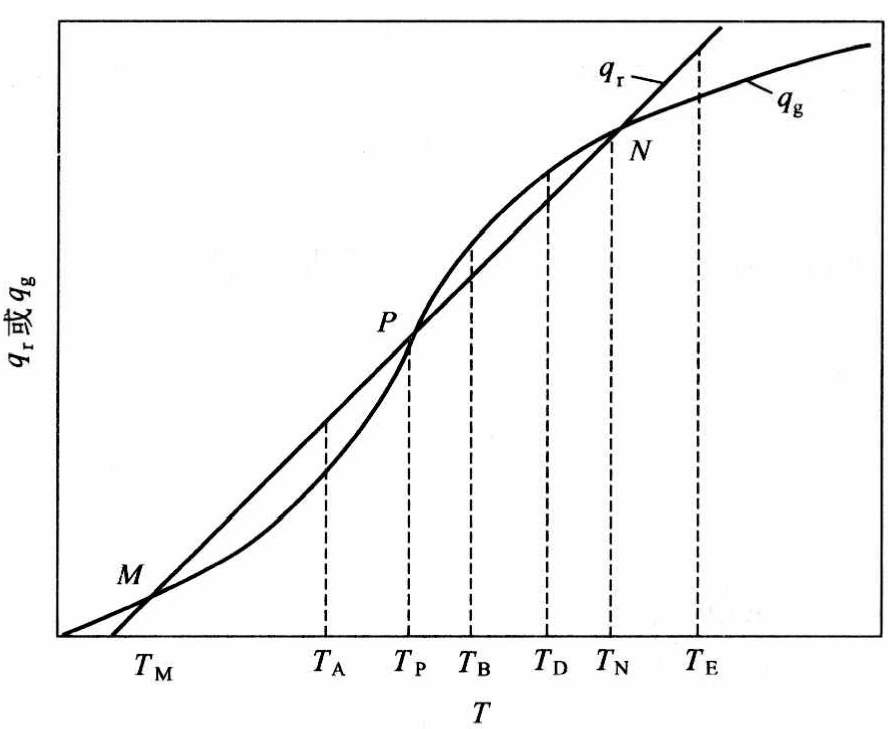
\includegraphics[width=\linewidth]{figs/fig3.13.png}
        \column{9.5cm}
            \begin{itemize}
            \item 移热速率线$q_\mathrm{r}$为一直线，斜率为$Q_{0} \rho \bar{C}_{p \mathrm{t}}+U A_{\mathrm{h}}$
            \item 放热速率曲线$q_\mathrm{g}$为一S形曲线
            \item 两线的交点的温度即为定态操作温度
            \end{itemize}        
    \end{columns}
\end{frame}


\begin{frame}
    \frametitle{连续釜式反应器的定态}

    \begin{columns}[c]
        \column{6cm}
            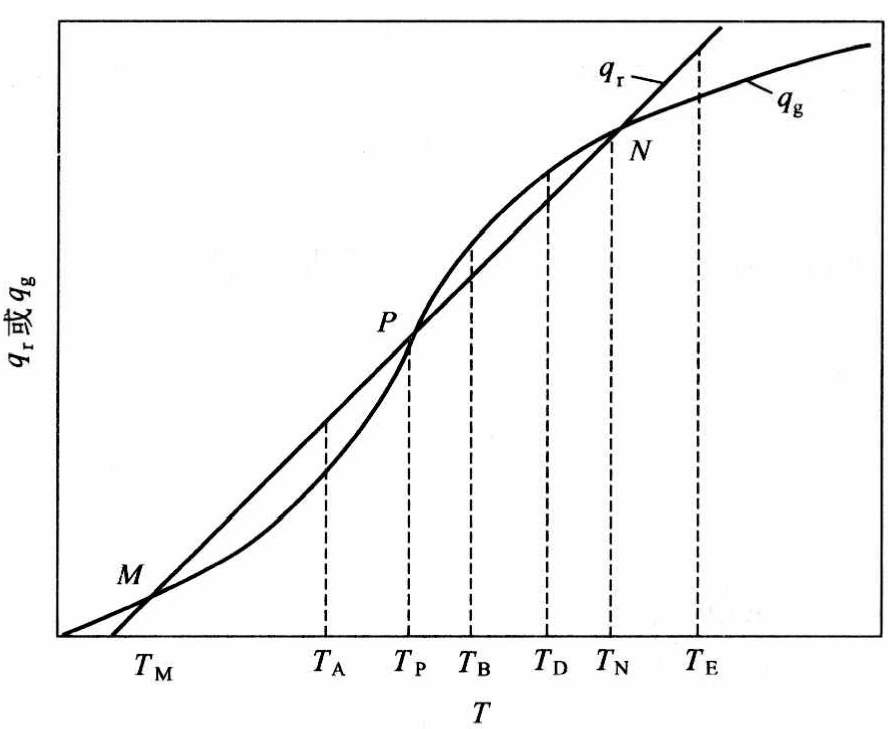
\includegraphics[width=\linewidth]{figs/fig3.13.png}
        \column{7.5cm}
            \begin{itemize}
            \item $T_\mathrm{M}$、$T_\mathrm{N}$、$T_\mathrm{P}$为定态操作温度
            \item 按$T_\mathrm{M}$操作，转化率最低，按$T_\mathrm{N}$操作，转化率最高            
            \item M、N为稳定定态点
            \item P为不稳定的定态点
            \item 只有放热反应才可能出现多定态现象，吸热反应的定态总是唯一的
            \end{itemize}        
    \end{columns}
    ~\\
    以N点为例，当受到外来干扰温度上升至$T_\mathrm{E}$，此时移热速率大于放热速率，扰动消除后，反应物系必然降温至$T_\mathrm{N}$。如由于外来干扰温度下降至$T_\mathrm{D}$，此时$q_\mathrm{r}$大于$q_\mathrm{g}$，扰动消除后，反应物系必然升温至$T_\mathrm{N}$。所以N是稳定定态点。

\end{frame}


\begin{frame}
    \frametitle{连续釜式反应器的着火点和熄火点}
    当进料流量一定且传热系数及反应物料的比热容可视为常数时，进料或换热介质温度改变只使移热曲线的位置发生变化，而不影响放热曲线。
    \vspace{6pt} 
    \begin{columns}[c]        
        \column{5.5cm}
        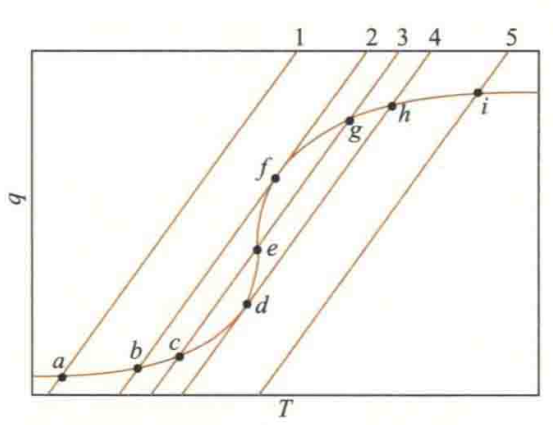
\includegraphics[width=\linewidth]{figs/fig3.14a.png}
        \centering 进料温度不同时的定态点
        \column{8cm}
        当进料温度从$T_1$慢慢地增加到$T_4$时，定态温度从点$a$变至$d$，该点为不稳定的定态点，只要进料温度稍微增加，定态点即从点$d$跳至点$h$出现不连续现象。这种情况称为着火，点d称为着火点。

        如逐渐降低进料温度，点$f$为不稳定的定态点，定态点将从点$f$跳至点$b$。这种情况称为熄火，点$d$称为熄火点。
    \end{columns}
\end{frame}


\begin{frame}
    \frametitle{连续釜式反应器的着火点和熄火点}
    \begin{columns}[c]
        \column{8cm}
            如图为进料温度$T_0$与定态温度$T$的关系示意图。
            
            当进料温度从$T_1$慢慢地增加至$T_5$时，定态温度的变化$a\rightarrow b\rightarrow c\rightarrow d\rightarrow h\rightarrow i$。
            
            曲线在$d$点处是不连续的，定态温度突然增高，这一点称为着火点；

            若将进料温度逐渐降低，比如从$T_5$降至$T_1$，定态温度则沿$i\rightarrow h\rightarrow g\rightarrow f\rightarrow b\rightarrow a$曲线下降。间断点$f$称为熄火点。
        \column{5.5cm}
            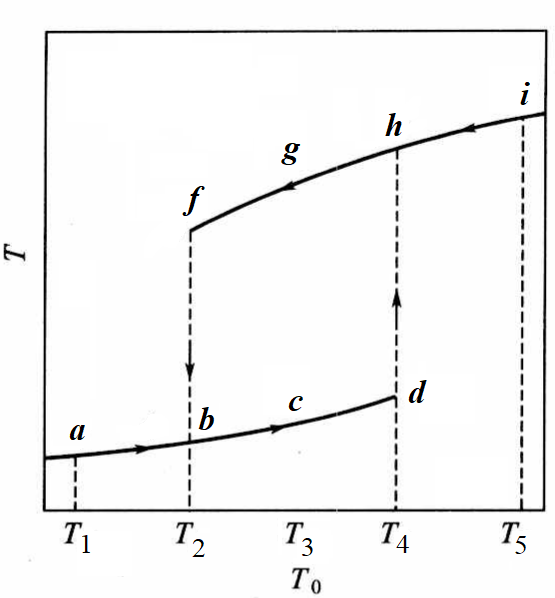
\includegraphics[width=\linewidth]{figs/fig3.14.png}
    \end{columns}    
    当进料温度在$T_2$与$T_4$的范围内时，则产生多定态现象。在此温度范围之外，定态温度是唯一的。
\end{frame}


\begin{frame}[t]{}
    \begin{example}
        温度为326K的顺丁烯二酸酐和正己醇的混合液，以\SI{0.01}{m^3/s}的流量连续地通入反应体积为\SI{2.65}{m^3}的绝热釜式反应器进行酯化反应
        \[
            \ce{C4H2O3 + C6H13OH -> HOOC-CH=CH-COO(C6H13)}
        \]
        该反应对顺丁烯二酸酐和正己醇均为一级，反应速率常数等于
        \[
            k = 1.37 \times 10^{12} \exp{(-12628/T)} \qquad \mathrm{m^3/(kmol \cdot s)}
        \]
        该反应的反应热为\SI{-33.5}{kJ/mol}，反应混合物的$\rho \bar{C}_{p \mathrm{t}}$可按\SI{1980}{kJ/(m^3.K)}计算。

        进料液中酐和醇的浓度分别为\SI{4.55}{kmol/m^3}和\SI{5.34}{kmol/m^3}，试计算反应器出口转化率及温度。
    \end{example}

\end{frame}